\documentclass[noacm,sigplan]{acmart}

% \acmSubmissionID{PAPER ID}
\renewcommand\footnotetextcopyrightpermission[1]{}
\settopmatter{printfolios=false,printacmref=false}

\usepackage{setspace}
\usepackage{enumerate}
\usepackage{algorithm2e}
\usepackage{algpseudocode}
\usepackage{graphics}
\usepackage{xparse} 
\usepackage{xspace}
\usepackage{multirow}
\usepackage{csvsimple}
\usepackage{balance}
\usepackage{minted}
\usepackage{xcolor}
\usepackage{nicefrac}
\usepackage{siunitx}
\usepackage{array,framed}
\usepackage{booktabs}
\usepackage{color}
\usepackage{soul}
\usepackage{float}
\usepackage{epsfig}
\usepackage{wrapfig}
\usepackage{graphics}
\usepackage{graphicx}
\usepackage{subcaption}
\usepackage{adjustbox}
\usepackage{csquotes}
\usepackage{cleveref}
\usepackage{dirtytalk}
\usepackage{textgreek}

\def\eg{{\em e.g.}, }
\def\ie{{\em i.e.}, }
\def\etc{{\em etc.}\xspace}
\def\vs{{\em vs.}\xspace}

\def\gptmodel{{GPT-4o}\xspace}

\newcommand{\todo}[1]{\hl{\textbf{TODO:} #1}\xspace}
\newcommand{\sys}{{\scshape Kv{\textalpha}sir}\xspace}
\newcommand{\rf}[1]{\ref{#1}}
\newcommand{\sx}[1]{(\S\ref{#1})}
\newcommand{\cf}[1]{(\emph{Cf}.\S\ref{#1})}
\newcommand{\se}[1]{\S\ref{#1}}
\newcommand{\fg}[1]{Fig.~\ref{#1}}
\newcommand{\heading}[1]{\vspace{2pt}\noindent\textbf{\emph{#1}}:\enspace}
\newcommand{\ttt}[1]{\texttt{#1}\xspace}
\newcommand{\xxx}{\colorbox{red!30}{xxx}\xspace}
\newcommand{\promptbox}[1]{\hspace*{-0.0135\columnwidth}\fbox{\parbox[t]{0.95\columnwidth}{\tt{#1}}}}

\crefformat{section}{\S#2#1#3}
\crefmultiformat{section}{\S#2#1#3}{--\S#2#1#3}{, \S#2#1#3}{ and \S#2#1#3}

\begin{document}


\title{\sys: Controllable Program Regeneration}
\author{Evangelos Lamprou}


% Use cases for something like this include:
% - program repair
% - turning insecure code into secure code by removing side-effects
% - transforming a program in language A to language B
% - turning a program into a more idiomatic version of the same language
% - having a program use a different API
% - have a program be more amendable to parallelization
% - have a program be more amendable to further analysis or transformation

\begin{abstract}
Modern software systems are constantly evolving—requiring developers to
  refactor legacy code, adapt to changing APIs, translate across languages, and
  patch security vulnerabilities. These transformations are often brittle,
  manual, and error-prone. Large language models (LLMs) offer new opportunities
  for automating such tasks, but their outputs are shaped by surface cues, lack
  semantic guarantees, and require brittle prompting strategies. This paper
  presents \sys, a system for controllable program regeneration that combines
  logic-based planning with LLM-guided synthesis.
  By expressing transformation
  goals as declarative constraints over program properties---such as input/output
  behavior, side-effect freedom, language, or modular structure, \sys
  regenerates code that satisfies explicit semantic requirements.
  We demonstrate \sys across a wide range of tasks, including security
  hardening, language translation, and idiomatic rewriting, and highlight its
  ability to deliver interpretable, high-quality transformations with minimal
  developer guidance.
\end{abstract}
\maketitle

\section{Introduction}
\begin{figure}[t]
  % https://docs.google.com/drawings/d/1LAmdVYjfAID24eSM-hl5PRhVg9fRMJMWYETsvvcyAuU/edit?usp=sharing
  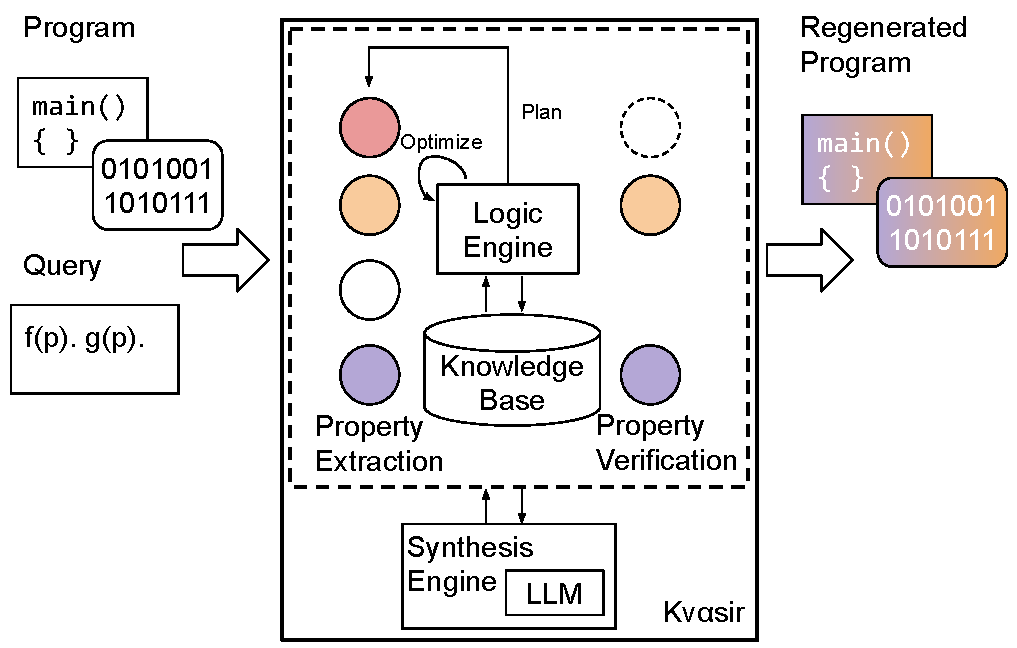
\includegraphics[width=\columnwidth]{figs/kvasir_overview.pdf}
  \caption{\textbf{\sys overview}
Given a transformation query, and a source program, \sys extracts a minimal set
  of properties,
  guided by a logic engine and knowledge base.
  It then synthesizes a new program $P'$ that satisfies the query, verifying
  that wanted properties are present and unwanted properties are absent in $P'$.
}
\end{figure}


% insights: modular programs, advances in LLMs, need for a strictly declarative interface

% Mention that:
% 1. They have shown great promise in program synthesis + 
% 2. They can not do negative reasoning well - 
% 3. Their output are often closely aligned to their inputs. They are gullible (susceptible to adversarial inputs). -
% 4. Difficult to verify correctness of outputs against certain properties. The
%    user cannot easily set requirements or say output should be within a range of
%    acceptance


Modern software systems evolve constantly.
Developers refactor legacy code~\cite{Fowler99,Mens04,facebook2010redesigns,dropbox2014syncengine},
adapt libraries to changing APIs~\cite{dig2005role,kula2017empiricalstudyimpactrefactoring},
translate components across languages~\cite{manzoor_cli_python,gaultier_rewrite_cpp},
and patch security vulnerabilities~\cite{ikegami2022userefactoringsecurityvulnerability,schneier2013security_vulnerabilities}.
These transformations, are often brittle, time-consuming, and require significant expertise.

Recent advances in large language models (LLMs) have opened new possibilities for automating program transformation and synthesis tasks, making them attractive tools for software evolution, albeit with caveats.
This flexibility has positioned them as attractive tools for software evolution.
LLMs can translate code across languages~\cite{ou2025enhancingllmbasedcodetranslation},
refactor complex modules~\cite{ziftci2025migrating},
and even generate entire components from scratch~\cite{huynh2025largelanguagemodelscode}.
However, surface-level patterns in the input shape their outputs~\cite{yang2025evaluatinggeneralizationcapabilitieslarge},
they struggle with negative constraints~\cite{hwang2024thinkpinkelephant,jiang2024llmsdreamelephantswhen},
often overfit to spurious input cues~\cite{xu2023llmfoolitselfpromptbased, wu2023deceptpromptexploitingllmdrivencode},
and lack mechanisms for enforcing precise behavioral properties on the generated code~\cite{roh2025breakthechainreasoningfailuresllms}.
As a result, developers must prompt and steer them through brittle heuristics or manual trial-and-error, leading to workflows that are difficult to audit, integrate, or systematically reason about.
Bridging this gap calls for a declarative interface---one that allows developers to specify explicit semantic constraints and transformation goals, and to reason about their satisfaction in a principled way.

This paper present \sys, a system for \emph{controllable program regeneration}.
\sys allows users
to express transformation goals declaratively, as logical constraints over
program properties such as input/output behavior, side-effect freedom, target
language, trace equivalence, or modular structure.
Given a source program and
such a query, \sys extracts a minimal set of relevant properties, guided by a
logic engine and a domain-specific knowledge base, and synthesizes a new
program that satisfies the desired constraints.

Three key insights shape the design of \sys.
First, modern software is highly modular, making it feasible to reason about transformations at the granularity of individual components or functions.
Second, the program regeneration setting provides a unique advantage: the original program serves as a concrete ground-truth, enabling semantic comparisons and verification of the transformed output, something impossible in traditional synthesis tasks.
Third, the underlying synthesis technology---particularly LLMs---is evolving rapidly; a declarative interface that harnesses this progress without disrupting the framework's end user.

Guided by these insights, \sys casts transformation as a constrained synthesis problem.
At its core is a property-driven pipeline: users express goals as logical constraints over semantic properties, such as input/output behavior, side-effect freedom, target language, or structural modularity.
\sys extracts a set of relevant properties, derived from its logic engine and a domain-aware knowledge base, and synthesizes a new program that satisfies the specified constraints.
If no such program exists, \sys returns a failure explanation from the unsatisfiable core.

\heading{Deployment scenarios and limitations}
\sys supports a range of deployment scenarios.
It is particularly well-suited for use during maintenance and auditing phases, where developers seek to refactor or replace components, especially when the original code is difficult to understand, modify, or is unavailable and the component exists only as a binary.
It can also assist during development, for instance when integrating third-party modules that must be adapted to local conventions or hardened against security vulnerabilities.
However, \sys is not designed for whole-program synthesis or large-scale migrations.
Its strength lies in scoped regeneration tasks, typically at the granularity of a function, method, or small module---where transformation goals can be explicitly stated and verified in isolation.
To this end, \sys functions not only as a standalone tool but also as a
library, where other components can invoke it as a programmable,
constraint-guided regeneration module.

% Leverages insights: (1) modern applications highly modular (2) the problem of LLM-assisted program transformations needs to be transformed in a way that a ground truth is readily available: the original program
% (3) towards the generality and longevity of this solution the interface needs to be purely declarative, to allow independent progress of the underlying comopnents to give automatic benefits

% TODO: Add section references
\heading{Contributions}
The paper's contributions are:
\begin{itemize}
  \item A property-aware transformation framework, combining logic-based reasoning, and LLM-assisted program synthesis~(\cref{sec:design});
 \item A declarative interface and accompanying DSL for program transformation, allowing users to express semantic goals as logical queries over properties of the regenerated program~(\cref{sec:dsl});
 \item A verification architecture that checks synthesized programs against the specified properties, providing feedback for refinement~(\cref{sec:verification});
 \item An empirical evaluation demonstrating \sys's effectiveness and scalability across transformation scenarios~(\cref{sec:evaluation}).
\end{itemize}

We evaluate \sys across a diverse set of transformation tasks~(\cref{sec:evaluation}), including:
	security hardening, by stripping latent malicious behavior while preserving intended functionality;
	cross-language translation, by regenerating semantically equivalent programs in new languages;
	idiomatic rewriting, by producing safer and more portable variants of legacy code;
	modular decomposition, by restructuring monolithic components into composable parts.
\sys is able to effectively regenerate programs across these tasks, producing high-quality outputs that satisfy user-specified constraints while also discovering transformation strategies that were not immediately obvious to the authors.

\heading{Availability}
The \sys prototype in available as an open-source MIT-licensed artifact at:
\begin{center}
  \url{https://github.com/vagos/kvasir}
\end{center}

\section{Example}
\label{sec:example}
\sys enables users to specify transformation goals declaratively.
Logical constraints over properties of the
regenerated program express these goals. Examples are input-output equivalence, side-effect elimination,
target language, lines of code, and others.

Given a program and a query over desired properties, \sys selects a minimal set
of properties to extract from the original program, then attempts to synthesize
a new program that satisfies the query.
\sys casts this process as a
maximum-satisfiability (MaxSAT) problem~\cite{sung2006maximum}, optimizing for the smallest extraction
effort necessary to enable transformation.
If the query is unsatisfiable under
the constraints or transformations, \sys issues an error
message, showing the conflict.

This section shows the application of \sys
to three distinct program transformation tasks, 
targeting security, language translation, compatibility,
idiomaticity, and modularity.

\heading{A compromised javascript library}
The \texttt{flatmap-stream} library was implicated in a high-profile
supply-chain attack that exfiltrated Bitcoin credentials~\cite{ev:eurosec:2022}.
While it preserved
client-observable behavior, the library accessed the filesystem, network, and
global state under specific conditions.
Program regeneration can automatically remove possible malicious payloads
while preserving the original program's observable behavior,
especially in this scenario, where the attack is highly obfuscated and 
activates under precise conditions~\cite{harp:ccs:2021}.
\begin{minted}[frame=lines]{js}
module.exports = function (stream, fn) {
 if (process.env.PRODUCTION) {
  const priv = copay.getKeys()?.[0]?.priv;
  if (priv && wallet.balance > 0) {
    http.request({ hostname: 'evil.com' })
        .send({ priv });
  }} return flatten(steam).apply(fn); };
\end{minted}

\begin{wrapfigure}[3]{r}{.5\columnwidth}
\vspace{-10pt}
\begin{minted}{prolog}
equal(graph(P), graph(P_)).
pure(P_).
\end{minted}
\end{wrapfigure}
To the right is a program written in the \sys DSL to express this intent.
This query requires the regenerated program \ttt{P\_} to exhibit the same I/O behavior,
but forbids side-effects.
\sys first arrives at a minimal set of properties to extract from the
original program, given its knowledge base and the query.
This set is $\{\texttt{funcs(F, P), graph(F), sig(F), pure(P)}\}$, where
\texttt{funcs(F, P)} extracts the set of functions defined in the original program
using a language-aware component that either parses the program source or extracts
symbols from the binary,
\texttt{graph(F)} extracts the I/O behavior of each function
by providing its source code to an LLM instance and asking it to generate a set of
inputs; with corresponding outputs generated by executing the original program,
and \texttt{sig(F)} extracts each function's signature.
The, \texttt{pure(P)} property means that \sys will confirm after regeneration that the original program is (obviously) pure
using static analysis.

After 30.4 seconds and one attempt, \sys generates the following program:
\begin{minted}[frame=lines]{js}
module.exports = function(stream, fn) {
  return stream.map(fn); };
\end{minted}


Building on the same source, \sys can perform cross-language
translation. 
Here, the goal is to regenerate a semantically equivalent version
of \texttt{flatmap-stream} in Haskell, to enable integration with a
Haskell-based pipeline or facilitate formal reasoning.

\begin{wrapfigure}[3]{r}{.5\columnwidth}
\vspace{-10pt}
\begin{minted}{prolog}
equal(graph(P), graph(P_)).
language(P_, haskell).
\end{minted}
\end{wrapfigure}
The query requests preservation of I/O behavior and translation to Haskell. The
logic engine deduces that extracting I/O traces and the function signature is
sufficient; the knowledge base automatically associates the target language
\texttt{Haskell} with purity.
\sys transforms each extracted I/O example into an equivalent one in Haskell (\eg 
the pair $\langle\texttt{([1,[2,3]], (x)=>x+1)}\to\texttt{[2,3,4]}\rangle$ 
becomes $\langle(\texttt{[1, [2,3]], Js("(x)=>x+1"))}\to\texttt{[2,3,4]}\rangle$).
Finally, it provides the transformed examples to a new LLM instance, prompting it
to generate a Haskell program that satisfies the same I/O behavior.
After 32.2 seconds, having generated 20 I/O pairs, \sys produces the following
Haskell program (truncated for brevity):
\begin{minted}[frame=lines]{haskell}
flatmap :: (a -> b) -> NestedList a -> [b]
flatmap f (Elem x) = [f x]
flatmap f (List x) = concatMap (flatmap f) x
\end{minted}

\heading{An unidiomatic c program}
The fast inverse square root routine from the Quake III
engine~\cite{fast_inv_sqrt}
is a classic example of performance-oriented low-level programming.
The original implementation exploits type punning to manipulate IEEE
floats at the bit level---an optimization that relies on undefined behavior:

\begin{minted}[frame=lines]{c}
float Q_rsqrt(float number) {
 long i; float x2, y;
 const float threehalfs = 1.5F;
 x2 = number * 0.5F; y  = number;
 i  = * ( long * ) &y; // evil bit level hack
 i  = 0x5f3759df - ( i >> 1 );
 y  = * ( float * ) &i;
 y  = y * ( threehalfs - ( x2 * y * y ) );
 return y;
}
\end{minted}

The following query for \sys uses lines-of-code a coarse metric of
idiomaticity. \sys will regenerate the program, minimizing this metric, while
preserving its I/O behavior.
\begin{wrapfigure}[3]{r}{.5\columnwidth}
  \vspace{-5pt}
  \begin{minted}{prolog}
equal(graph(P), graph(P_)).
#min len(P_).
  \end{minted}
\end{wrapfigure}
\sys extracts the set of properties \ttt{sig(F)} and \ttt{graph(F)} from the original program, where \texttt{sig(F)} is the
signature of the function (including its name, return type, and arguments), and \texttt{graph(F)} is the I/O behavior of the function
on a set of generated inputs.
In this case, where the goal is to optimize an aspect of the program, \sys will re-prompt
the model to regenerate the program until it can make no improvements or there is a negligible difference after two consecutive iterations.
After 15.2 seconds, and two iterations, \sys produces the following program:
\begin{minted}[frame=lines]{c}
#include <math.h>
float Q_rsqrt(float number) {
    return 1.0f / sqrtf(number);
}
\end{minted}
The regenerated version is easier to verify, portable across compilers, and
avoids undefined behavior.
A user could have also provided performance requirements using 
the \ttt{time(P)} property to further guide the regeneration process.
In this case, \sys would have run the two functions inside a tight loop and 
would have aborted the regeneration process if the performance of the generated
program was not within an acceptable user-defined threshold.

\heading{A rigid music application}
Consider a JavaScript application that retrieves and displays a user's music
collection from an SQLite database~\cite{codewithsadeemusicplayer, beets}:

\begin{minted}[frame=lines]{js}
function getAlbumsByArtist(artist) {
  const db = new Database("music.db");
  const rows = db.prepare("SELECT album
  FROM songs WHERE artist = ?").all(artist);
  return rows.map(row => row.album); }
\end{minted}

Having the database initialization being in the same function as 
the database access has architectural and performance implications.
In addition, there exist systems that can benefit from further decomposition
of an application towards automatic distribution, parallelization or security~\cite{Towards_Modern_Ghemaw_2023, vasilakis2019ignis, vasilakis2018breakapp}.
\begin{wrapfigure}[5]{r}{.7\columnwidth}
  \vspace{-10pt}
  \begin{minted}{prolog}
db('music.db').
equal(trace(P,sql),trace(P_,sql)).
func(F1). func(F2).
equal(F2(F1, _), P).
\end{minted}
\end{wrapfigure}
\sys, given the query to the right, will 
generate program that consists of two functions,
whose composition is equivalent to the original program, and feature 
the same I/O and trace properties (a trace here being the sequence of SQL 
queries transmitted to the database).
\sys wraps the node process with monitors that extract the SQL queries 
sent to the database for 24 generated inputs.
Then, after 20.4 seconds and two attempts, it arrives at two functions $f_1$, and 
$f_2$, where their composition $f_2(f_1, \_)$, is equivalent to the original \ttt{getAlbumsByArtist} function across these inputs.
A final processing step renames functions $f_1$ and $f_2$ by prompting an LLM instance.
Alternatively, the user could have provided specific signatures and names for each 
functions as an additional guiding property.
The resulting program is:
\begin{minted}[frame=lines]{js}
function connectDB() {
 const sqlite = require('sqlite');
 return sqlite.open({filename: 'music.db'}); }
function getAlbumsByArtist(db, artist) {
 const rows = await db.all("SELECT album
 FROM songs WHERE artist = ?", artist);
 return rows.map(row => row.album); }
\end{minted}

% \heading{Key results}
% \sys is able to effectively transform programs across a variety goals.

\section{\sys Design}
\label{sec:design}

% \sys is a system for program regeneration: given an input program and a set of
% behavioral, structural, or syntactic properties, it synthesizes a new program
% that satisfies a specified subset of those properties. The system treats
% regeneration as a goal-driven process, guided by explicit property
% specifications and a symbolic planner that structures the search space for a
% backend synthesizer.
At a high level, \sys operates in four phases: (1) plan construction, (2)
property extraction, (3) program synthesis, and (4) verification and feedback.
These phases interact through a shared representation of the program and its
transformation goals.

\heading{Plan construction}
First, each of the available plugins contributes a set of pre and pos-conditions 
to the logic engine.
Essentially, these describe what needs to hold for an analysis to be applicable to the given 
program and what properties \sys will preserve or transform after regeneration.
Then, the planning component accepts one or more user-provided regeneration goals (termed as the query).
The full set of rules and predicates are used to construct an ASP program
a solver then accepts.
From the solver's output, the planner constructs a plan that specifies which
analysies \sys plugins should apply to the input program and what properties can be
preserved during regeneration in order to fullfill the query.

\heading{Property extraction} \sys then continues by analyzing the input program to
extract the collection of properties.
These may describe the program's interface
(\eg, exported functions), its operational constraints (\eg, disallowing
filesystem access), or its structure (\eg, use of a particular API or programming idiom).
While some properties are derived from generic analyses
applicable across languages~(\eg examples of input-output behavior), others are specific to the input program's language and runtime model.

\heading{Synthesis}
Guided by the transformation plan, \sys creates a prompt template which is then
augmented with the extracted properties, having them normalized to a human-readable text represantation.
This prompt is then passed to an LLM instance.
\sys does not include by default the original program's source code in the prompt.
Instead, it uses the extracted properties to guide the LLM instance 
to synthesize a candidate program that satisfies the specified constraints.

\heading{Verification and feedback}
The final phase verifies that the
synthesized program satisfies the target properties.
If verification fails---due to a violated constraint or behavioral divergence---\sys uses this
failure as a signal to refine the plan or resample the synthesis step.
This forms a feedback loop: planning, synthesis, and verification interact until \sys
produces a satisfactory program or the system exhausts its search.

\section{Property Language and Extraction}
\label{sec:dsl}

\sys represents program characteristics as symbolic \emph{properties}, drawn from a language of first-order predicates.
These properties describe aspects of the input program and serve as regeneration constraints for the output.
They form the basis of both planning and verification.
All aspects of the symbolic representation are expressed as answer-set programming (ASP) facts and rules (an example program is shown in \cref{lst:logic-example})~\cite{Eiter_2009}.

\heading{Property predicates}
Each property is a logical predicate over the program symbol $p$. Common examples include:
\begin{itemize}
  \item \texttt{language}$(p, \texttt{javascript})$: the input program is written in JavaScript.
  \item \texttt{signature}$(p)$: the program exposes a well-formed function signature.
  \item \texttt{pure}$(p)$: the program does not have side-effects (\eg file system access, network calls, \etc).
\end{itemize}

Properties fall into three categories:
\begin{itemize}
  \item $\mathsf{goal}(X)$: the user requires $X$ to hold in the regenerated program. The system derives such facts from the user query.
  \item $\mathsf{can}(X)$: the system is capable of extracting or inferring property $X$ from the input. Plugins add these facts and represent the system's capabilities.
  \item $\mathsf{do}(X)$: $X$ the planner selects $X$ for enforcement and the synthesizer will preserve or regenerate it. 
\end{itemize}

\heading{Planning over properties}
The logic engine determines the set of active properties to enforce by solving a constrained optimization problem over $\mathsf{do}(\cdot)$. It satisfies the following constraints:
\begin{align*}
  \mathsf{goal}(X) &\Rightarrow \mathsf{do}(X) &\text{Satisfy all goals} \\
  \mathsf{do}(X) &\Leftarrow \mathsf{can}(X) &\text{Apply only extractable properties}
\end{align*}
\sys also supports minimization, maximization and elimination of properties
through the $\mathsf{goal\_min}$, $\mathsf{goal\_max}$, and $\mathsf{goal\_not}$ and the corresponding $\mathsf{do\_min}$, $\mathsf{do\_max}$, and $\mathsf{do\_not}$ predicates.
Without loss of generality, the text encompasses the four cases under $\mathsf{goal}$ and $\mathsf{do}$, explicitly mentioning the rest when there is an important semantic difference.

Additionally, the system maximizes the number of extracted properties:
\[
\text{maximize} \left|\left\{ X \mid \mathsf{do}(X) \right\}\right|
\]
Essentially, the planner tries to give the synthesizer as much information
as possible, as long as it doesn't violate any regeneration goals.

\heading{Plugin-defined rules}
Plugins contribute domain-specific inference rules and constraints. For example, a plugin for JavaScript-to-Haskell translation may define:
\begin{align*}
\mathsf{can}(\texttt{translate}_{\texttt{js} \rightarrow \texttt{hs}}(p)) & \\
\mathsf{do}(\texttt{translate}_{\texttt{js} \rightarrow \texttt{hs}}(p)) &\Rightarrow \mathsf{do}(\texttt{language}(p, \texttt{haskell})) \\
\mathsf{do}(\texttt{translate}_{\texttt{js} \rightarrow \texttt{hs}}(p)) &\Rightarrow \mathsf{language}(p, \texttt{javascript})
\end{align*}
Another plugin might contribute $\mathsf{can}(\texttt{signature}(p))$, indicating it can extract the function signature. At this stage, \sys only cares about semantics of each plugin in relation to how it might enable or violate 
other properties in the regenerated program.

\heading{Axioms and domain knowledge}
The logic engine also includes domain-wide axioms based on some common assumptions.
For example
$\mathsf{do}(\texttt{language}(p, \texttt{haskell})) \Rightarrow \mathsf{do}(\texttt{pure}(p))$
captures the assumption that programs written in Haskell are pure by default.
Such axioms allow inferred properties to trigger downstream constraints or synthesis behaviors.

\begin{listing}
  \begin{minted}[frame=lines, fontsize=\small]{prolog}
language(p, c).
can(len(p)). % len plugin
can(signature(p)). % signature plugin
can(js2hs(p)). % js2hs plugin
do(language(p, haskell)) :- do(js2hs(p)).
:- do(js2hs(p)), not language(p, javascript).

% Core solver logic
:- do(language(p, X)), language(p, Y), X != Y,
    not goal(language(p, X)).
{ do(X) } :- can(X), not goal_min(X).
{ do_min(X) } :- can(X).
ndo(N) :- N = #count { X : do(X) }.
#maximize { N : ndo(N) }.
:- goal(X), not do(X).
:- goal_min(X), not do_min(X).
:- do(language(P, L1)), do(language(P, L2)), L1 != L2.

goal_min(len(p)). % User query
\end{minted}
  \caption{\textbf{Example \sys logic program.}
  This is a lightly simplified version of the logic program that produces the plan for the idiomatization task~(\cref{sec:example}). 
  The program contains facts coming from (1) the input program (written in C),
  (2) three plugins (\ttt{len}, \ttt{signature}, and \ttt{javascript2haskell}),
  (3) axioms from the logic engine (\eg a program can have one language, an analysis will be applied only if possible, all goals must be satisfied), and
  (4) the user query (the user wants to minimize the length of the program).
  }
  \label{lst:logic-example}
\end{listing}

\heading{Extensibility}
\sys decentralizes property extraction: plugins contribute $\mathsf{can}(\cdot)$ facts, and pre- and post-conditions, while the core planner resolves which properties to enforce based on goals, capabilities, and axioms.
This modularity allows language-specific analyses to coexist with general-purpose reasoning in a unified planning layer.

\section{Synthesis Plan}
\label{sec:synthesis}

The synthesis process begins with a set of enforced properties $\{ X \mid \mathsf{do}(X) \}$
which the planner selected~(\cref{sec:dsl}).
These properties
reflect both user goals (\eg removing side effects, translating to a
different language) and structural characteristics of the input program that
the synthesizer will preserve.
The planner constructs a transformation plan that
specifies, for each relevant unit of code (typically a function), what
constraints must hold in the regenerated version.

For instance, a plan for regenerating a specific function $f$ might include:
\(\mathsf{do}(\texttt{language}(f, \texttt{haskell}))\) the function must be written in Haskell, 
\(\mathsf{do}(\texttt{pure}(f))\) the function must be side-effect-free, and 
\(\mathsf{do}(\texttt{signature}(f))\) the function must keep its signature.

\heading{LLM-guided regeneration}
A structured prompt guides the language model, which performs the synthesis task.
The prompt is a composition of natural-language text fragments plugins contribute. 
A plugin can include domain-specific instructions as further guidance.
For example:
A \ttt{signature} plugin may contribute:

 \promptbox{
   {The output should implement a function \texttt{sqrt(n: float): float}.}
 }
A \ttt{length} plugin combined with a minimization goal may prepend:

\promptbox{
  {The output should be as short as possible while preserving the original functionality.}
}
A \ttt{javascript2haskell} plugin may prepend:

\promptbox{
  {The output function should be written in Haskell.}
}

These fragments, combined with a normalized text representations of each of 
the extracted properties constitute the prompt given to the LLM.

\heading{Constraint-guided generation}
While \sys delegates code synthesis to a large language model, the planner constrains the generation space in two key ways.
First, the prompt instructs the LLM to perform only transformations that are valid under the current plan.
For instance, if the target function must be pure, the prompt will exclude information such as system-call traces that might imply side-effectful behavior.
Second, candidate outputs are verified post hoc against the enforced properties~(\cref{sec:verification}).
% This hybrid model balances flexibility with rigor: the LLM provides diversity and fluency, while the planner ensures adherence to property-based constraints.

\section{Property Verification and Feedback Loop}
\label{sec:verification}

To validate that a regenerated program satisfies the intended goals, \sys includes an explicit verification phase that checks whether the output adheres to the enforced properties in the synthesis plan. 
Verification accepts only programs that meet the plan's constraints and provides feedback for refining or retrying those that do not.

\heading{Verification as property checking}
After synthesis, \sys invokes a set of property-specific checkers. Each checker is responsible for evaluating whether a property $X$ in $\mathsf{do}(X)$ holds for the regenerated program fragment. These checkers operate at varying levels of precision---ranging from structural pattern checks to light static or symbolic analysis---and are tailored to the property type.

Examples include:
\begin{itemize}
  \item For $\mathsf{do}(\texttt{no\_network}(f))$, the checker confirms the absence of known network APIs or imports.
  \item For $\mathsf{do}(\texttt{signature}(f))$, the checker matches the regenerated function's name, parameters, and arity against the extracted signature.
  \item For $\mathsf{do}(\texttt{pure}(f))$, the checker examines control flow and side-effecting operations to detect possible violations.
\end{itemize}

Checkers are modular and contributed by plugins. Their combined results determine whether a candidate is considered valid under the current plan.
For minimization and maximization goals, the verification phase uses the less-than or greater-than operators as are defined internally by the plugin verifying the given property.
Verfication in this case checks if the property's value has decreased or increased compared 
to the previous regeneration attempt.
If the value remains unchanged for two consecutive attempts, its considered satisfied.

\heading{Failure-driven refinement}
When a candidate fails verification, \sys treats this as a feedback signal. Instead of discarding the regeneration attempt wholesale, the system uses the failure to revise or re-execute the synthesis phase.
Some forms are:
\begin{itemize}
  \item \emph{Retrying synthesis}: A fresh LLM call with the same plan but a different generation path.
  \item \emph{Feedback loop}: \sys will provide the previous regeneration attempt 
    as an additional context to the LLM, together with an explanation of the properties that the regeneration violates, prompting it to adapt its output based on prior failures.
    This mode is only activated if the verifier knows that the output will not to taint
    followupp regeneration attempts.
  \item \emph{Fallback handling}: If a function repeatedly fails validation, \sys may leave the original version intact or mark it for manual inspection.
\end{itemize}

% This loop provides adaptability: regeneration is not expected to succeed unconditionally, but rather to proceed incrementally under interpretable, bounded failure modes.

\heading{Partial regeneration and composition}
\sys supports regeneration at the granularity of individual functions.
If only a subset of functions can be successfully regenerated under the given constraints, the remaining ones remain unchanged after regeneration.
The output program thus consists of a composition of validated regenerated units and untouched originals.
This model supports application in real-world codebases, where partial improvement (\eg replacing unsafe or deprecated functions) can be meaningful even without complete coverage.

\section{Evaluation}
\label{sec:evaluation}

We evaluate \sys along three axes:

\begin{itemize}
  \item[\textbf{Q1}] \textbf{Correctness and Regeneration Quality}: Does \sys preserve program behavior and produce high-quality programs?
  \item[\textbf{Q2}] \textbf{LLM Baseline}: How does \sys compare to naively prompting a large language model?
  \item[\textbf{Q3}] \textbf{Planning Efficiency \& Precision}: Does minimizing extracted properties help regeneration succeed faster and more reliably?
    % TODO: Maybe make naive LLM Q3 and merge Q3 and Q2.
\end{itemize}

\subsection{Benchmarks \& Methodology}

We evaluate \sys on six benchmark suites, summarized in \cref{tab:benchmarks}.
Each task consists of an input program, a \sys query expressing desired
properties, and a test suite or functional oracle.
The Rosetta Code~\cite{rosettacode} benchmarks include four programming tasks written in four different
languages each (Python, JavaScript, C, and Haskell). 
These include classic programs that do not require any language-specific features to implement.
These are: the classic \emph{Hello, World!} program as found in most programming tutorials,
a program that applies the ROT-13 cipher to a string,
a program that computes the median of a list of numbers,
and a program that reads a file and prints its contents to the console line-by-line.
The npm benchmark includes ten popular (100.000+ weekly downloads) npm packages that implement utility
functionality such as string manipulation, data structure transformations, and math.
Similalry, the PyPi utilities benchmark includes three functions sourced from PyPi that implement similar functionality.
The SSCA dataset includes three sneaky supply-chain attacks that obfuscate malicious behavior in otherwise innocuous-looking code.
The attack activates under specific environment conditions, such as the presence of a specific environment variable or specific inputs
getting passed to the program. The attacks involve private key exfiltration~\cite{ohm2020backstabber}, Bitcoin private key theft~\cite{ev:eurosec:2022}, and an SSH backdoor installation~\cite{copeland2019frightening}.
and occur while the program still performs its advertised functionality.
The IOCCC benchmark includes two programs from the International Obfuscated C Code Contest (IOCCC)~\cite{ioccc}.
These programs are intentionally obfuscated, using advanced techniques such as bit manipulation, undefined behavior,
and exploitation of the C preprocessor and the lax parsing rules of the C language.
These programs perform mathematical computations like mersense primality testing and adding two numbers.
Finally, the microbenchmarks include three programs that implement the regeneration tasks discussed in \cref{sec:example}.

\begin{table}[h]
\centering
  \caption{\textbf{Benchmark summary}. 
  Benchmark programs come from online repositories, public archives, security research datasets, and often referenced examples in programming culture.
  The $N$ column shows the number of programs/functions from each benchmar.
  }
\begin{tabular}{llrl}
\toprule
Benchmark                          & Description         & $N$ & Source \\
\midrule
Rosetta Code                       & Programming tasks   & 16   & \cite{rosettacode} \\
npm utilities                      & Utilities from npm  & 10  & \cite{regbench2025} \\
PyPi utilities                   & Utilities from PyPi & 3   & \cite{regbench2025} \\
SSCA                               & Sneaky SSAs         & 3   & \cite{ev:eurosec:2022, ohm2020backstabber,copeland2019frightening} \\
IOCCC                              & Obfuscated C code   & 2   & \cite{ioccc} \\
Microbenchmarks                    &                     & 3   & \\
\hspace{.5em} \ttt{flatmap-stream} & Secure regeneration &     & \cite{es1}  \\
\hspace{.5em} \ttt{Q\_rsqrt}       & C refactoring       &     & \cite{fast_inv_sqrt}  \\
\hspace{.5em} \textsf{rigidDB}     & Modularization      &     & \cite{codewithsadeemusicplayer} \\
\bottomrule
\end{tabular}
\label{tab:benchmarks}
\end{table}

\subsection{Q1: Correctness and Regeneration Quality}

We evaluate correctness using developer-made test suites 
shipped with the original software components as well as by manually inspecting
the regenerated source code and report on correctness and the other query target metrics.
When no test suite is available, we only do manual inspection.

\begin{table}[h]
  \centering
  \caption{Correctness: Percentage of tasks passing all tests (when present) and manual inspection.}
  \begin{tabular}{lc}
    \toprule
    Benchmark & \sys Pass Rate \\ 
    \midrule
    Rosetta Code & 16/16  \\
    npm Utilities & 10/10 \\
    Python Utilities & 3/3\\
    SSCA & 3/3  \\
    IOCCC & 1/2 \\
    Microbenchmarks & 2.5/3  \\
    \bottomrule
  \end{tabular}
\end{table}

\sys succeeds in all of the Rosetta Code benchmarks, code is correct, we had to manually verify it as no test cases are available.
\sys regenerates correctly all npm and PyPi utilities, it does not introduce and sideffectful or malicious behavior.
The synthesized programs reveal several interesting insights and patterns.
\sys-generated code often lacks the optimizations commonly
implemented by library developers, such as early exits or caching.
For instance, the \texttt{left-pad} library, precomputes padding for strings below a certain length
and returns it directly. In contrast, \sys tends to produce straightforward
implementations without attempting similar optimizations.
\sys also omits domain-specific knowledge.
For example, in the \texttt{is} family of libraries,
\sys-generated code frequently fails to account for all edge cases,
and often misses JavaScript-specific patterns,
such as checking an object’s string representation to decide if an object is circular, as in the \texttt{is-circular} library.
\sys has weak performance on libraries that involve complex regexes or perform non-trivial math.
For the SSCA benchmarks, \sys successfully regenerates all three malicious libraries, removing the malicious behavior while preserving the original functionality.
For the flatmap-stream attack, \sys uses some domain-specific logic (encoded in its knowledge-base by the \ttt{js-stream} plugin) to generate a function that produces a node \ttt{Stream} object.
For the IOCCC benchmarks, \sys regenerates the \ttt{adder} program, which is a simple program that adds two numbers,
it also regenerates \ttt{mersenne} in regards that it correctly performs a naive mersenne primality testing, but it does not follow the non-obvious output scheme of the original program, which returns a non-zero hexadecimal number when $2^p - 1$ ($p$ being the input number) is not prime.
For the microbenchmarks, \sys correctly regenerates the \ttt{flatmap-stream} program, producing a safe Haskell version that is idiomatic and preserves the original functionality.
However, this version does not match exactly the semantics of the original one, as it operates over infinitely nested lists, rather than only one level deep ones.
The \ttt{Q\_rsqrt} program includes the obvious, idiomatic computation of the inverse square root ($1/\sqrt{x}$) rather than the original bit-level manipulation.
Finally, \sys successfully decomposes the \ttt{rigidDB} program into two
functions, \ttt{setupDatabase} and \ttt{getAlbumsByArtist}, which is a
modularization that preserves the original functionality and produce equivalent I/O and SQL traces.

\sys is able to regenerate programs that are correct and preserve the original functionality,
while also removing any malicious behavior or obfuscation.
Failure cases highlight current limitations, and inspire future work~(\cref{sec:discussion}).

\subsection{Q2: Naive LLM vs. \sys}

To compare \sys against a baseline, we use a \gptmodel instance
that performs prompt-only rewriting without explicit access to guiding properties.
The LLM gets the following prompt template:

\promptbox{
  \emph{Task description} \eg {Give back the same code having removed any vulnuerabilities}\\

  Program:\\
  \emph{Program/function source code}\\

  Please return the program's source code after performing the task.
}

For the Rosetta Code benchmarks, \gptmodel 
succesful in all language translation tasks.
The original and LLM-generated code matches the semantics
of the original one, confirmed after manually inspecting the generated code.
Similarly, the LLM was succesful in transforming the npm and PyPi utilities towards
removing any vulnerabilities from them, as they are benign and the transformation
involved the LLM simply repeating the original code without any changes.
The SSCA benchmark tasks are more interesting, as they involve 
malicious code. For the malicious libraries, we provide the LLM 
with two different versions. One is the original high-profile attack that appeared on npm,
with the second one being an attack that is semantically equivalent but with the source 
having gone through an iterative loop where a second LLM is tasked with making the code ostensibly 
secure. This involves adding integrity checks at all points in the program where a value is used.
\gptmodel was succesful in eliminating the original attacks, but failed in \emph{all} 
cases where the source code was particulalry crafted to appear secure, regenerating both 
the original functionality and the attack.
For the IOCCC benchmarks, \gptmodel also fails 
in both cases to regenerate the programs in a way where the code's 
functionality is preserved while removing the obfuscation.
The \ttt{adder} program is regenerated as a program that prints the \ttt{argc} argument, 
while the \ttt{mersenne} program performs irrelevant arithmetic operations that 
resemble the original source, and fails to even compile.
For the microbenchmarks, \gptmodel is able to regenerate the \ttt{flatmap-stream} program, but fails to produce a Haskell version of it,
as it overfits to the original JavaScript source code which uses the \ttt{Stream} API,
and fails to produce a Haskell program that is nor equivalent to the original, nor idiomatic.
For the \ttt{Q\_rsqrt} program, \gptmodel fails to produces a program that idiomatically 
computes the inverse square root, rather trying to minimize the number of lines in the program
by removing constants and comments and still keeping the bit-level manipulation.
Finally, for the \ttt{rigidDB} program, \gptmodel is able to decompose the original program into two functions
and names them \ttt{setupDatabase} and \ttt{getAlbumsByArtist}.

\sys consistently outperforms a \gptmodel baseline,
highlighting the inherent weaknesses of a purely prompt-based approach.

\subsection{Q3: Planning Efficiency \& Precision}

To evaluate the impact of \sys's property planning, we compare it against a \gptmodel baseline that performs prompt-only rewriting without explicit access to guiding properties.

We consider two criteria for each regenerated program:

\begin{itemize}
  \item \textbf{Wanted Property Satisfaction:} Does the output program satisfy all positive properties declared in the query (\eg \texttt{pure}, \texttt{language(haskell)})?
  \item \textbf{Unwanted Property Avoidance:} Does the output avoid introducing disallowed behaviors (\eg side effects, global state, unsupported language features)?
\end{itemize}

\sys consistently satisfies more of the declared properties while avoiding
unintended behaviors. For instance, in the \texttt{flatmap-stream} benchmark,
\gptmodel often inclduded malicious side effects when the code appeared innocuous,
whereas \sys generated pure rewrites by treating the source as
untrusted and grounding regeneration in I/O behavior alone.
Across all benchmarks, the planning step completes in under 50ms on average.
Similalry, in the \ttt{Q\_rsqrt} benchmark, \gptmodel often produces bit-level
manipulations that are not idiomatic in Haskell, while \sys generates a simple
and idiomatic Haskell function that computes the inverse square root.
This is guided by the fact the \sys extracts and provides to its backend model only the function signature 
and length of the program, which it minimizes, without including the original source code,
which as shown in the experimental results makes the model overfit its regeneration to it.
\sys's I/O pair extraction also provides confidence that 
the regenerated program has the same client-visible behavior as the original one, while 
prompting a model like \gptmodel would always require manual inspection or the presence 
of developer tests to verify the correctness of the regeneration.

These results support the claim that \sys's planning logic---driven by explicit
property extraction and knowledge-base reasoning---yields safer and more
controllable transformations than prompt-only LLM-based systems.

\section{Related Work}

\heading{Program synthesis}
Program synthesis research spans a rich space of techniques.
Classical techniques emphasize correctness and
interpretability, synthesizing programs from specifications~\cite{alur2013syntax, feser2015synthesizing, gulwani2011automating},
type constraints \cite{polikarpova2016program},
or examples \cite{jha2010oracle, raza2018disjunctive, singh2016blinkfill}.
These works often target narrowly
defined domains such as string manipulation~\cite{harp:ccs:2021} or data migration
\cite{yaghmazadeh2018automated} and focus on ensuring provable guarantees.
More recently, LLM-based methods~\cite{austin2021program, chen2021evaluating}
explore broad-domain code generation via prompt-based conditioning.
While flexible, these models are prone to hallucination and struggle
with reasoning under negation or satisfying structured constraints~\cite{xu2023llmfoolitselfpromptbased, wu2023deceptpromptexploitingllmdrivencode,jiang2024llmsdreamelephantswhen,hwang2024thinkpinkelephant}.

\sys leverages insights from both these paradigms.
Unlike purely symbolic or purely neural approaches, it leverages LLMs within a
constrained planning framework to guide transformations while remaining
responsive to property-based requirements.
This design combines
the scalability of LLM-assisted program sysnthesis with the controllability and robustness of symbolic
reasoning. % TODO: focus on that \sys focuses on this specific problem domain

\heading{Program transformations and refactoring}
The evolution and maintenance of software systems often involve transformations
such as refactoring, translation, or security hardening. Foundational work on
refactoring~\cite{Fowler99} and its taxonomy~\cite{Mens04} characterizes the
space of behavior-preserving modifications. More recent perspectives emphasize
developer experience and usability, particularly in the context of APIs~\cite{Myers16}.

Tools in this space often operate via syntax-tree transformations or
domain-specific templates. Verification-based methods such as \textsc{Dafny}
\cite{Leino10} and \textsc{CBMC} \cite{Clarke04} ensure functional correctness
but require heavy formalization.
Others automate migration via
programming-by-example or interactive guidance \cite{gulwani2017program, le2017interactive}.

Kvasir aims to generalize this landscape by treating transformations as
goal-directed regenerations---rather than prescriptive rewrites, driven by
properties such as program behaviors and architectural goals, expressed declaratively.

\heading{Logic programming and constraint solving}
Logic programming has long served as a foundation for reasoning in programming
tools, offering a declarative model for expressing properties and constraints.
Answer Set Programming (ASP), in particular, provides a rich framework for
expressing defaults, exceptions, and optimization via stable model semantics
\cite{Gelfond_2000, Gelfond_2002, Eiter_2009}. 
ASP has been used for
declarative program analysis \cite{benton2007interactive}, automated planning
\cite{nguyen2020explainable, son2022answersetplanningsurvey}, and knowledge
representation in verification and synthesis pipelines.

\sys uses ASP as its planning back-end for the planning, decision-making
process, while also uses its straighftorward optimization capabilities.
For each transformation task, \sys formulates the property-satisfaction problem as a logic query and uses an ASP solver to
synthesize a feasible transformation plans.
This enables global reasoning across program components and enforces
user-specified constraints that are difficult for neural models to respect.
In addition, it offers a level of explainability that is useful in case transformations end up incorrect.

\section{Discussion and Limitations}
\label{sec:discussion}

\sys supports property-guided regeneration of program fragments, with a particular focus on function-level rewrites. Its strength lies in combining symbolic reasoning and generative synthesis in a modular and interpretable framework. However, this design comes with inherent tradeoffs.

\heading{Targeted regeneration}
\sys is best used as a surgical tool for targeted regeneration tasks, not for whole-program synthesis or full language migration.
It operates most effectively on localized units of code---such as individual functions, methods, or small modules, where behavior is self-contained and transformation goals can be expressed through explicit constraints.
% Typical applications include rewriting high-risk, deprecated, or poorly understood code segments where correctness is critical and semantic preservation is essential.
Broad, untargeted use may yield incomplete results and can be bottlenecked by the limited context of the back-end model \sys uses.

\heading{Dependence on property specification}
The system relies heavily on the quality and granularity of extracted or declared properties.
In cases where desired behaviors cannot be easily expressed using available predicates, or where plugins fail to extract meaningful constraints, the regeneration plan may be under-constrained, leading to brittle or incorrect outputs. The framework is extensible, but each new property class requires the development of a new plugin that will provide a set of pre- and post-conditions, an extractor, and a verifier.

\heading{Trust model and correctness}
\sys
does not provide formal guarantees
of semantic equivalence
to the original program.
Instead,
correctness is defined relative to a set of enforced properties.
This means that correctness is only as strong as the property definitions and associated verifiers.
In the presence of underspecified or unverifiable goals,
regenerated code
may exhibit unanticipated behavior,
even if it passes all checks. 


\heading{LLM limitations}
The generative synthesis phase
is subject to the inherent variability and failure modes
of large language models.
These include hallucinations,
sensitivity to prompt phrasing,
and inconsistency
under minor input changes.
\sys does not mitigate these risks,
but allows their detection
through post-hoc verification.
In cases where the system finds no satisfactory candidate,
regeneration fails.


\heading{Language-specific support}
Although some components of \sys are language-agnostic (\eg logic-based planning),
others---particularly extraction and verification plugins are not.
Supporting a new language
requires implementing language-specific analyzers and constraints.
This modularity is deliberate,
but it does limit out-of-the-box generality.
Work on a unified language representation~\cite{koppel2018onetool,bap2011,dillig2009sail},
is relevant to overcomming this limitation.
The current \sys prototype
supports Python, JavaScript, Haskell, and C. 


\heading{Future directions}
Extensions that could improve \sys's capabilities include richer property languages (\eg temporal or dataflow properties~\cite{azzopardi2023ltl,handa2021orderawaredataflowmodelparallel}), tighter integration with formal verification tools, and cross-component reasoning for coordinated rewrites.
Furthermore, performance-oriented transformations could be potent additions, allowing \sys to transform the program across dimensions like runtime, parallelizability, or memory usage.
Additionally, integrating counterfactual generation techniques~\cite{Cabalar_2020} could help explain why certain regeneration goals are infeasible or conflicting.

% Overall, \sys offers a flexible framework for controlled regeneration, but its effectiveness depends on the specificity of goals, the availability of property logic, and the scope of the transformation task. Its design favors composability and clarity over full automation, aiming to serve as a building block in broader refactoring, auditing, or hardening pipelines.

\section{Conclusion}
This paper introduced \sys, a system for property-guided program regeneration
that bridges the flexibility of large language models with the precision of
logic-driven planning.
By allowing developers to declaratively specify
transformation goals as logical constraints, \sys elevates LLM-assisted program
trasnformations to a controllable, interpretable, and iterative synthesis-verification
process.
Evaluation demonstrates that \sys produces high-quality regenerations
across diverse tasks, outperforming naive prompting baselines in correctness,
controllability, and resilience to adversarial or obfuscated inputs.

\sys opens the door to a new class of synthesis tools that combine symbolic
reasoning and neural generation under a unified, extensible framework.
As program synthesis systems grow increasingly reliant on LLMs, we believe the
future lies in harnessing their generative power within a framework that retains
correctness, explainability, and developer control as first-class citizens.


\bibliographystyle{ACM-Reference-Format}
\bibliography{bib.bib}

\end{document}
